\documentclass[twoside]{book}

% Packages required by doxygen
\usepackage{fixltx2e}
\usepackage{calc}
\usepackage{doxygen}
\usepackage[export]{adjustbox} % also loads graphicx
\usepackage{graphicx}
\usepackage[utf8]{inputenc}
\usepackage{makeidx}
\usepackage{multicol}
\usepackage{multirow}
\PassOptionsToPackage{warn}{textcomp}
\usepackage{textcomp}
\usepackage[nointegrals]{wasysym}
\usepackage[table]{xcolor}

% Font selection
\usepackage[T1]{fontenc}
\usepackage[scaled=.90]{helvet}
\usepackage{courier}
\usepackage{amssymb}
\usepackage{sectsty}
\renewcommand{\familydefault}{\sfdefault}
\allsectionsfont{%
  \fontseries{bc}\selectfont%
  \color{darkgray}%
}
\renewcommand{\DoxyLabelFont}{%
  \fontseries{bc}\selectfont%
  \color{darkgray}%
}
\newcommand{\+}{\discretionary{\mbox{\scriptsize$\hookleftarrow$}}{}{}}

% Page & text layout
\usepackage{geometry}
\geometry{%
  a4paper,%
  top=2.5cm,%
  bottom=2.5cm,%
  left=2.5cm,%
  right=2.5cm%
}
\tolerance=750
\hfuzz=15pt
\hbadness=750
\setlength{\emergencystretch}{15pt}
\setlength{\parindent}{0cm}
\setlength{\parskip}{3ex plus 2ex minus 2ex}
\makeatletter
\renewcommand{\paragraph}{%
  \@startsection{paragraph}{4}{0ex}{-1.0ex}{1.0ex}{%
    \normalfont\normalsize\bfseries\SS@parafont%
  }%
}
\renewcommand{\subparagraph}{%
  \@startsection{subparagraph}{5}{0ex}{-1.0ex}{1.0ex}{%
    \normalfont\normalsize\bfseries\SS@subparafont%
  }%
}
\makeatother

% Headers & footers
\usepackage{fancyhdr}
\pagestyle{fancyplain}
\fancyhead[LE]{\fancyplain{}{\bfseries\thepage}}
\fancyhead[CE]{\fancyplain{}{}}
\fancyhead[RE]{\fancyplain{}{\bfseries\leftmark}}
\fancyhead[LO]{\fancyplain{}{\bfseries\rightmark}}
\fancyhead[CO]{\fancyplain{}{}}
\fancyhead[RO]{\fancyplain{}{\bfseries\thepage}}
\fancyfoot[LE]{\fancyplain{}{}}
\fancyfoot[CE]{\fancyplain{}{}}
\fancyfoot[RE]{\fancyplain{}{\bfseries\scriptsize Generated by Doxygen }}
\fancyfoot[LO]{\fancyplain{}{\bfseries\scriptsize Generated by Doxygen }}
\fancyfoot[CO]{\fancyplain{}{}}
\fancyfoot[RO]{\fancyplain{}{}}
\renewcommand{\footrulewidth}{0.4pt}
\renewcommand{\chaptermark}[1]{%
  \markboth{#1}{}%
}
\renewcommand{\sectionmark}[1]{%
  \markright{\thesection\ #1}%
}

% Indices & bibliography
\usepackage{natbib}
\usepackage[titles]{tocloft}
\setcounter{tocdepth}{3}
\setcounter{secnumdepth}{5}
\makeindex

% Hyperlinks (required, but should be loaded last)
\usepackage{ifpdf}
\ifpdf
  \usepackage[pdftex,pagebackref=true]{hyperref}
\else
  \usepackage[ps2pdf,pagebackref=true]{hyperref}
\fi
\hypersetup{%
  colorlinks=true,%
  linkcolor=blue,%
  citecolor=blue,%
  unicode%
}

% Custom commands
\newcommand{\clearemptydoublepage}{%
  \newpage{\pagestyle{empty}\cleardoublepage}%
}

\usepackage{caption}
\captionsetup{labelsep=space,justification=centering,font={bf},singlelinecheck=off,skip=4pt,position=top}

%===== C O N T E N T S =====

\begin{document}

% Titlepage & ToC
\hypersetup{pageanchor=false,
             bookmarksnumbered=true,
             pdfencoding=unicode
            }
\pagenumbering{roman}
\begin{titlepage}
\vspace*{7cm}
\begin{center}%
{\Large print\+\_\+ip }\\
\vspace*{1cm}
{\large Generated by Doxygen 1.8.11}\\
\end{center}
\end{titlepage}
\clearemptydoublepage
\tableofcontents
\clearemptydoublepage
\pagenumbering{arabic}
\hypersetup{pageanchor=true}

%--- Begin generated contents ---
\chapter{otus-\/homewrok4}
\label{md_README}
\hypertarget{md_README}{}
\input{md_README}
\chapter{Hierarchical Index}
\section{Class Hierarchy}
This inheritance list is sorted roughly, but not completely, alphabetically\+:\begin{DoxyCompactList}
\item false\+\_\+type\begin{DoxyCompactList}
\item \contentsline{section}{container$<$ typename $>$}{\pageref{structcontainer}}{}
\item \contentsline{section}{is\+\_\+valid$<$ T, U $>$}{\pageref{structis__valid_3_01T_00_01U_01_4}}{}
\item \contentsline{section}{is\+\_\+valid$<$ T, U, tuple\+\_\+args... $>$}{\pageref{structis__valid_3_01T_00_01U_00_01tuple__args_8_8_8_01_4}}{}
\end{DoxyCompactList}
\item \contentsline{section}{is\+\_\+valid$<$ T, tuple\+\_\+args $>$}{\pageref{structis__valid}}{}
\item \contentsline{section}{is\+\_\+valid$<$ T, tuple\+\_\+args... $>$}{\pageref{structis__valid}}{}
\begin{DoxyCompactList}
\item \contentsline{section}{is\+\_\+valid$<$ T, T, tuple\+\_\+args... $>$}{\pageref{structis__valid_3_01T_00_01T_00_01tuple__args_8_8_8_01_4}}{}
\end{DoxyCompactList}
\item true\+\_\+type\begin{DoxyCompactList}
\item \contentsline{section}{container$<$ std\+:\+:list$<$ T, Args... $>$ $>$}{\pageref{structcontainer_3_01std_1_1list_3_01T_00_01Args_8_8_8_01_4_01_4}}{}
\item \contentsline{section}{container$<$ std\+:\+:vector$<$ T, Args... $>$ $>$}{\pageref{structcontainer_3_01std_1_1vector_3_01T_00_01Args_8_8_8_01_4_01_4}}{}
\item \contentsline{section}{is\+\_\+valid$<$ T $>$}{\pageref{structis__valid_3_01T_01_4}}{}
\item \contentsline{section}{is\+\_\+valid$<$ T, T $>$}{\pageref{structis__valid_3_01T_00_01T_01_4}}{}
\end{DoxyCompactList}
\end{DoxyCompactList}

\chapter{Class Index}
\section{Class List}
Here are the classes, structs, unions and interfaces with brief descriptions\+:\begin{DoxyCompactList}
\item\contentsline{section}{\hyperlink{structcontainer}{container$<$ typename $>$} }{\pageref{structcontainer}}{}
\item\contentsline{section}{\hyperlink{structcontainer_3_01std_1_1list_3_01T_00_01Args_8_8_8_01_4_01_4}{container$<$ std\+::list$<$ T, Args... $>$ $>$} }{\pageref{structcontainer_3_01std_1_1list_3_01T_00_01Args_8_8_8_01_4_01_4}}{}
\item\contentsline{section}{\hyperlink{structcontainer_3_01std_1_1vector_3_01T_00_01Args_8_8_8_01_4_01_4}{container$<$ std\+::vector$<$ T, Args... $>$ $>$} }{\pageref{structcontainer_3_01std_1_1vector_3_01T_00_01Args_8_8_8_01_4_01_4}}{}
\item\contentsline{section}{\hyperlink{structis__valid}{is\+\_\+valid$<$ T, tuple\+\_\+args $>$} }{\pageref{structis__valid}}{}
\item\contentsline{section}{\hyperlink{structis__valid_3_01T_01_4}{is\+\_\+valid$<$ T $>$} \\*Thank\textquotesingle{}s cxx17 standard }{\pageref{structis__valid_3_01T_01_4}}{}
\item\contentsline{section}{\hyperlink{structis__valid_3_01T_00_01T_01_4}{is\+\_\+valid$<$ T, T $>$} }{\pageref{structis__valid_3_01T_00_01T_01_4}}{}
\item\contentsline{section}{\hyperlink{structis__valid_3_01T_00_01T_00_01tuple__args_8_8_8_01_4}{is\+\_\+valid$<$ T, T, tuple\+\_\+args... $>$} }{\pageref{structis__valid_3_01T_00_01T_00_01tuple__args_8_8_8_01_4}}{}
\item\contentsline{section}{\hyperlink{structis__valid_3_01T_00_01U_01_4}{is\+\_\+valid$<$ T, U $>$} }{\pageref{structis__valid_3_01T_00_01U_01_4}}{}
\item\contentsline{section}{\hyperlink{structis__valid_3_01T_00_01U_00_01tuple__args_8_8_8_01_4}{is\+\_\+valid$<$ T, U, tuple\+\_\+args... $>$} }{\pageref{structis__valid_3_01T_00_01U_00_01tuple__args_8_8_8_01_4}}{}
\end{DoxyCompactList}

\chapter{File Index}
\section{File List}
Here is a list of all files with brief descriptions\+:\begin{DoxyCompactList}
\item\contentsline{section}{\hyperlink{print__ip_8cpp}{print\+\_\+ip.\+cpp} }{\pageref{print__ip_8cpp}}{}
\item\contentsline{section}{\hyperlink{print__ip_8h}{print\+\_\+ip.\+h} }{\pageref{print__ip_8h}}{}
\item\contentsline{section}{\hyperlink{test__version_8cpp}{test\+\_\+version.\+cpp} }{\pageref{test__version_8cpp}}{}
\item\contentsline{section}{\hyperlink{version_8h}{version.\+h} }{\pageref{version_8h}}{}
\item\contentsline{section}{\hyperlink{version__lib_8h}{version\+\_\+lib.\+h} }{\pageref{version__lib_8h}}{}
\end{DoxyCompactList}

\chapter{Class Documentation}
\hypertarget{structcontainer}{}\section{container$<$ typename $>$ Struct Template Reference}
\label{structcontainer}\index{container$<$ typename $>$@{container$<$ typename $>$}}


{\ttfamily \#include $<$print\+\_\+ip.\+h$>$}



Inheritance diagram for container$<$ typename $>$\+:
\nopagebreak
\begin{figure}[H]
\begin{center}
\leavevmode
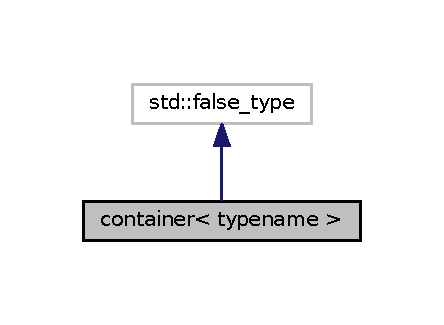
\includegraphics[width=213pt]{structcontainer__inherit__graph}
\end{center}
\end{figure}


Collaboration diagram for container$<$ typename $>$\+:
\nopagebreak
\begin{figure}[H]
\begin{center}
\leavevmode
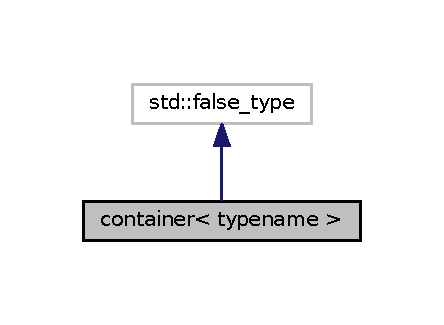
\includegraphics[width=213pt]{structcontainer__coll__graph}
\end{center}
\end{figure}


The documentation for this struct was generated from the following file\+:\begin{DoxyCompactItemize}
\item 
\hyperlink{print__ip_8h}{print\+\_\+ip.\+h}\end{DoxyCompactItemize}

\hypertarget{structcontainer_3_01std_1_1list_3_01T_00_01Args_8_8_8_01_4_01_4}{}\section{container$<$ std\+:\+:list$<$ T, Args... $>$ $>$ Struct Template Reference}
\label{structcontainer_3_01std_1_1list_3_01T_00_01Args_8_8_8_01_4_01_4}\index{container$<$ std\+::list$<$ T, Args... $>$ $>$@{container$<$ std\+::list$<$ T, Args... $>$ $>$}}


{\ttfamily \#include $<$print\+\_\+ip.\+h$>$}



Inheritance diagram for container$<$ std\+:\+:list$<$ T, Args... $>$ $>$\+:
\nopagebreak
\begin{figure}[H]
\begin{center}
\leavevmode
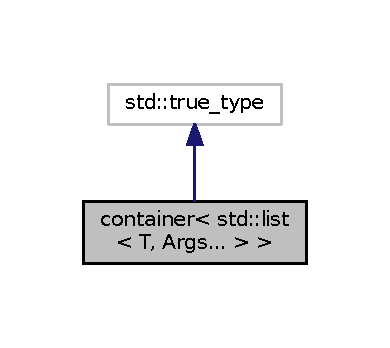
\includegraphics[width=187pt]{structcontainer_3_01std_1_1list_3_01T_00_01Args_8_8_8_01_4_01_4__inherit__graph}
\end{center}
\end{figure}


Collaboration diagram for container$<$ std\+:\+:list$<$ T, Args... $>$ $>$\+:
\nopagebreak
\begin{figure}[H]
\begin{center}
\leavevmode
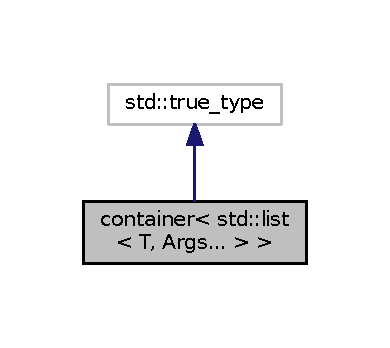
\includegraphics[width=187pt]{structcontainer_3_01std_1_1list_3_01T_00_01Args_8_8_8_01_4_01_4__coll__graph}
\end{center}
\end{figure}


The documentation for this struct was generated from the following file\+:\begin{DoxyCompactItemize}
\item 
\hyperlink{print__ip_8h}{print\+\_\+ip.\+h}\end{DoxyCompactItemize}

\hypertarget{structcontainer_3_01std_1_1vector_3_01T_00_01Args_8_8_8_01_4_01_4}{}\section{container$<$ std\+:\+:vector$<$ T, Args... $>$ $>$ Struct Template Reference}
\label{structcontainer_3_01std_1_1vector_3_01T_00_01Args_8_8_8_01_4_01_4}\index{container$<$ std\+::vector$<$ T, Args... $>$ $>$@{container$<$ std\+::vector$<$ T, Args... $>$ $>$}}


{\ttfamily \#include $<$print\+\_\+ip.\+h$>$}



Inheritance diagram for container$<$ std\+:\+:vector$<$ T, Args... $>$ $>$\+:
\nopagebreak
\begin{figure}[H]
\begin{center}
\leavevmode
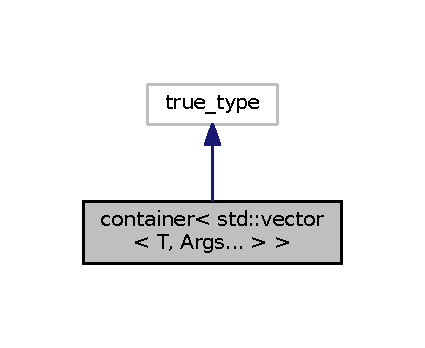
\includegraphics[width=204pt]{structcontainer_3_01std_1_1vector_3_01T_00_01Args_8_8_8_01_4_01_4__inherit__graph}
\end{center}
\end{figure}


Collaboration diagram for container$<$ std\+:\+:vector$<$ T, Args... $>$ $>$\+:
\nopagebreak
\begin{figure}[H]
\begin{center}
\leavevmode
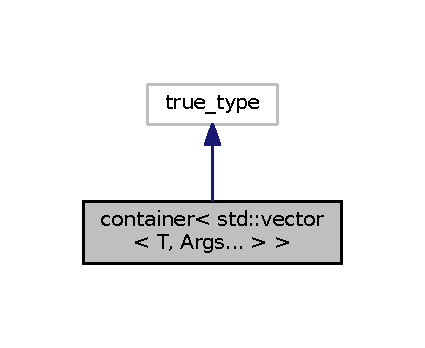
\includegraphics[width=204pt]{structcontainer_3_01std_1_1vector_3_01T_00_01Args_8_8_8_01_4_01_4__coll__graph}
\end{center}
\end{figure}


The documentation for this struct was generated from the following file\+:\begin{DoxyCompactItemize}
\item 
\hyperlink{print__ip_8h}{print\+\_\+ip.\+h}\end{DoxyCompactItemize}

\hypertarget{structis__valid}{}\section{is\+\_\+valid$<$ T, tuple\+\_\+args $>$ Struct Template Reference}
\label{structis__valid}\index{is\+\_\+valid$<$ T, tuple\+\_\+args $>$@{is\+\_\+valid$<$ T, tuple\+\_\+args $>$}}


{\ttfamily \#include $<$print\+\_\+ip.\+h$>$}



The documentation for this struct was generated from the following file\+:\begin{DoxyCompactItemize}
\item 
\hyperlink{print__ip_8h}{print\+\_\+ip.\+h}\end{DoxyCompactItemize}

\hypertarget{structis__valid_3_01T_01_4}{}\section{is\+\_\+valid$<$ T $>$ Struct Template Reference}
\label{structis__valid_3_01T_01_4}\index{is\+\_\+valid$<$ T $>$@{is\+\_\+valid$<$ T $>$}}


thank\textquotesingle{}s cxx17 standard  




{\ttfamily \#include $<$print\+\_\+ip.\+h$>$}



Inheritance diagram for is\+\_\+valid$<$ T $>$\+:
\nopagebreak
\begin{figure}[H]
\begin{center}
\leavevmode
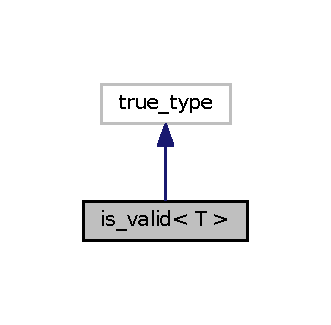
\includegraphics[width=159pt]{structis__valid_3_01T_01_4__inherit__graph}
\end{center}
\end{figure}


Collaboration diagram for is\+\_\+valid$<$ T $>$\+:
\nopagebreak
\begin{figure}[H]
\begin{center}
\leavevmode
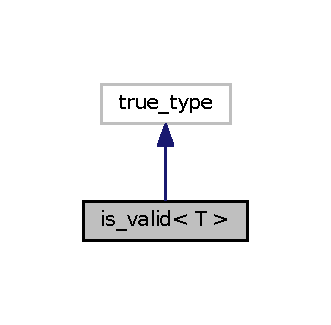
\includegraphics[width=159pt]{structis__valid_3_01T_01_4__coll__graph}
\end{center}
\end{figure}


\subsection{Detailed Description}
\subsubsection*{template$<$typename T$>$\\*
struct is\+\_\+valid$<$ T $>$}

thank\textquotesingle{}s cxx17 standard 

The documentation for this struct was generated from the following file\+:\begin{DoxyCompactItemize}
\item 
\hyperlink{print__ip_8h}{print\+\_\+ip.\+h}\end{DoxyCompactItemize}

\hypertarget{structis__valid_3_01T_00_01T_01_4}{}\section{is\+\_\+valid$<$ T, T $>$ Struct Template Reference}
\label{structis__valid_3_01T_00_01T_01_4}\index{is\+\_\+valid$<$ T, T $>$@{is\+\_\+valid$<$ T, T $>$}}


{\ttfamily \#include $<$print\+\_\+ip.\+h$>$}



Inheritance diagram for is\+\_\+valid$<$ T, T $>$\+:
\nopagebreak
\begin{figure}[H]
\begin{center}
\leavevmode
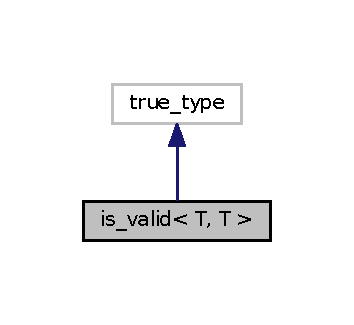
\includegraphics[width=170pt]{structis__valid_3_01T_00_01T_01_4__inherit__graph}
\end{center}
\end{figure}


Collaboration diagram for is\+\_\+valid$<$ T, T $>$\+:
\nopagebreak
\begin{figure}[H]
\begin{center}
\leavevmode
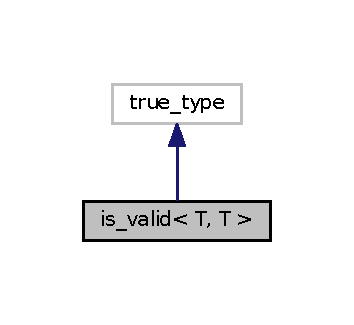
\includegraphics[width=170pt]{structis__valid_3_01T_00_01T_01_4__coll__graph}
\end{center}
\end{figure}


The documentation for this struct was generated from the following file\+:\begin{DoxyCompactItemize}
\item 
\hyperlink{print__ip_8h}{print\+\_\+ip.\+h}\end{DoxyCompactItemize}

\hypertarget{structis__valid_3_01T_00_01T_00_01tuple__args_8_8_8_01_4}{}\section{is\+\_\+valid$<$ T, T, tuple\+\_\+args... $>$ Struct Template Reference}
\label{structis__valid_3_01T_00_01T_00_01tuple__args_8_8_8_01_4}\index{is\+\_\+valid$<$ T, T, tuple\+\_\+args... $>$@{is\+\_\+valid$<$ T, T, tuple\+\_\+args... $>$}}


{\ttfamily \#include $<$print\+\_\+ip.\+h$>$}



Inheritance diagram for is\+\_\+valid$<$ T, T, tuple\+\_\+args... $>$\+:
\nopagebreak
\begin{figure}[H]
\begin{center}
\leavevmode
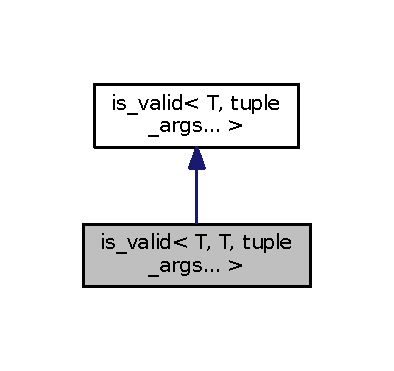
\includegraphics[width=189pt]{structis__valid_3_01T_00_01T_00_01tuple__args_8_8_8_01_4__inherit__graph}
\end{center}
\end{figure}


Collaboration diagram for is\+\_\+valid$<$ T, T, tuple\+\_\+args... $>$\+:
\nopagebreak
\begin{figure}[H]
\begin{center}
\leavevmode
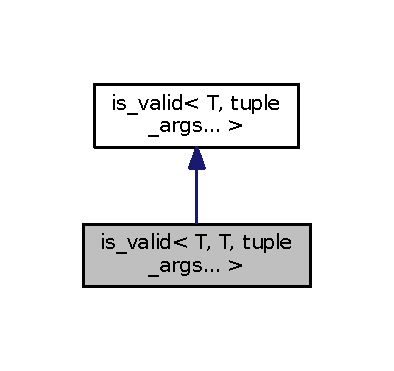
\includegraphics[width=189pt]{structis__valid_3_01T_00_01T_00_01tuple__args_8_8_8_01_4__coll__graph}
\end{center}
\end{figure}


The documentation for this struct was generated from the following file\+:\begin{DoxyCompactItemize}
\item 
\hyperlink{print__ip_8h}{print\+\_\+ip.\+h}\end{DoxyCompactItemize}

\hypertarget{structis__valid_3_01T_00_01U_01_4}{}\section{is\+\_\+valid$<$ T, U $>$ Struct Template Reference}
\label{structis__valid_3_01T_00_01U_01_4}\index{is\+\_\+valid$<$ T, U $>$@{is\+\_\+valid$<$ T, U $>$}}


{\ttfamily \#include $<$print\+\_\+ip.\+h$>$}



Inheritance diagram for is\+\_\+valid$<$ T, U $>$\+:
\nopagebreak
\begin{figure}[H]
\begin{center}
\leavevmode
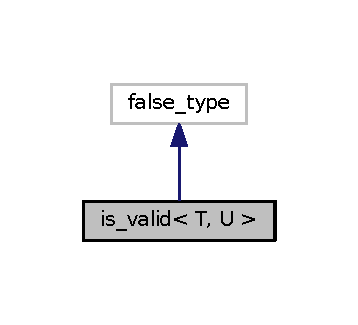
\includegraphics[width=172pt]{structis__valid_3_01T_00_01U_01_4__inherit__graph}
\end{center}
\end{figure}


Collaboration diagram for is\+\_\+valid$<$ T, U $>$\+:
\nopagebreak
\begin{figure}[H]
\begin{center}
\leavevmode
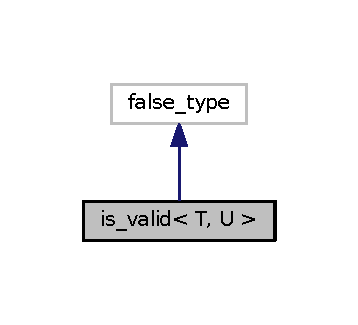
\includegraphics[width=172pt]{structis__valid_3_01T_00_01U_01_4__coll__graph}
\end{center}
\end{figure}


The documentation for this struct was generated from the following file\+:\begin{DoxyCompactItemize}
\item 
\hyperlink{print__ip_8h}{print\+\_\+ip.\+h}\end{DoxyCompactItemize}

\hypertarget{structis__valid_3_01T_00_01U_00_01tuple__args_8_8_8_01_4}{}\section{is\+\_\+valid$<$ T, U, tuple\+\_\+args... $>$ Struct Template Reference}
\label{structis__valid_3_01T_00_01U_00_01tuple__args_8_8_8_01_4}\index{is\+\_\+valid$<$ T, U, tuple\+\_\+args... $>$@{is\+\_\+valid$<$ T, U, tuple\+\_\+args... $>$}}


{\ttfamily \#include $<$print\+\_\+ip.\+h$>$}



Inheritance diagram for is\+\_\+valid$<$ T, U, tuple\+\_\+args... $>$\+:
\nopagebreak
\begin{figure}[H]
\begin{center}
\leavevmode
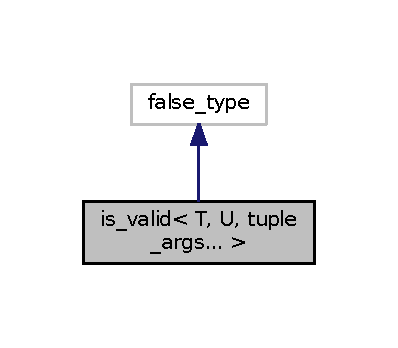
\includegraphics[width=191pt]{structis__valid_3_01T_00_01U_00_01tuple__args_8_8_8_01_4__inherit__graph}
\end{center}
\end{figure}


Collaboration diagram for is\+\_\+valid$<$ T, U, tuple\+\_\+args... $>$\+:
\nopagebreak
\begin{figure}[H]
\begin{center}
\leavevmode
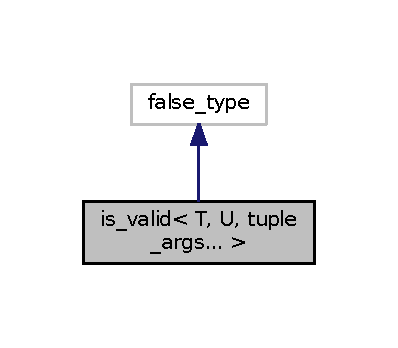
\includegraphics[width=191pt]{structis__valid_3_01T_00_01U_00_01tuple__args_8_8_8_01_4__coll__graph}
\end{center}
\end{figure}


The documentation for this struct was generated from the following file\+:\begin{DoxyCompactItemize}
\item 
\hyperlink{print__ip_8h}{print\+\_\+ip.\+h}\end{DoxyCompactItemize}

\chapter{File Documentation}
\hypertarget{print__ip_8cpp}{}\section{print\+\_\+ip.\+cpp File Reference}
\label{print__ip_8cpp}\index{print\+\_\+ip.\+cpp@{print\+\_\+ip.\+cpp}}
{\ttfamily \#include $<$iostream$>$}\\*
{\ttfamily \#include $<$vector$>$}\\*
{\ttfamily \#include $<$list$>$}\\*
{\ttfamily \#include $<$tuple$>$}\\*
{\ttfamily \#include \char`\"{}print\+\_\+ip.\+h\char`\"{}}\\*
Include dependency graph for print\+\_\+ip.\+cpp\+:
\nopagebreak
\begin{figure}[H]
\begin{center}
\leavevmode
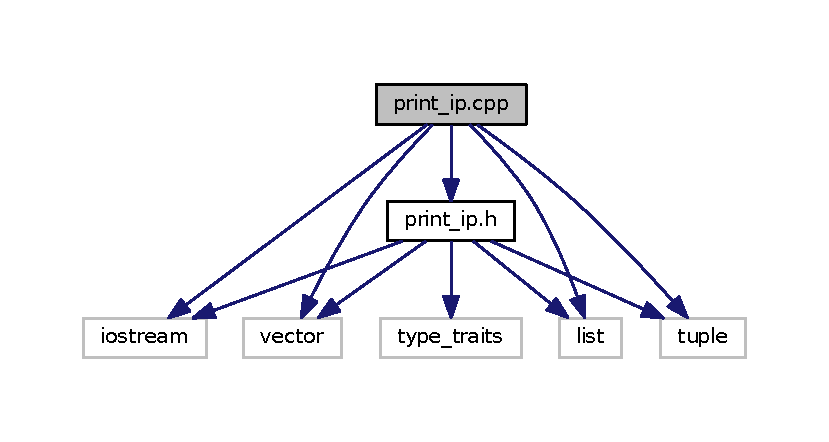
\includegraphics[width=350pt]{print__ip_8cpp__incl}
\end{center}
\end{figure}
\subsection*{Functions}
\begin{DoxyCompactItemize}
\item 
int \hyperlink{print__ip_8cpp_ae66f6b31b5ad750f1fe042a706a4e3d4}{main} ()
\end{DoxyCompactItemize}
\subsection*{Variables}
\begin{DoxyCompactItemize}
\item 
std\+::vector$<$ int $>$ \hyperlink{print__ip_8cpp_a84a7c734235ca6fee4fbcda505061957}{\+\_\+vector} \{110,111,112,113\}
\item 
std\+::list$<$ int $>$ \hyperlink{print__ip_8cpp_a224e3ccfe6cbec573ce05a626e5000ce}{\+\_\+list} \{99,98,97,96\}
\item 
std\+::string \hyperlink{print__ip_8cpp_a7d4d8ad0bbd0af8f510c05812ee5cb36}{\+\_\+string} \{\char`\"{}87.\+88.\+89.\+90\char`\"{}\}
\item 
const int \hyperlink{print__ip_8cpp_ae22be0a4fe9f5eaa17bc5daf5ac2ca27}{\+\_\+int} = 2130706433
\item 
const long long \hyperlink{print__ip_8cpp_a1adb27693f7573d27dcaba5e020717dc}{\+\_\+long} = 8875824491850138409
\item 
const unsigned short \hyperlink{print__ip_8cpp_ac57857a107fc58376edcb9c2b229b2f6}{\+\_\+short} = 0
\item 
const char \hyperlink{print__ip_8cpp_ab1d079a2b3af271a6d39da34541c36c5}{\+\_\+char} = -\/1
\item 
auto \hyperlink{print__ip_8cpp_ae9ae314de04458b92af76712b52f71c8}{\+\_\+tuple} = std\+::make\+\_\+tuple(\char`\"{}121\char`\"{},\char`\"{}125\char`\"{},\char`\"{}255\char`\"{},\char`\"{}254\char`\"{})
\item 
auto \hyperlink{print__ip_8cpp_a2cfe8d4a44ccf594b3427392b18a774a}{\+\_\+tuple\+\_\+bad} = std\+::make\+\_\+tuple(\char`\"{}1\char`\"{},\textquotesingle{}1\textquotesingle{},2, 4. )
\end{DoxyCompactItemize}


\subsection{Function Documentation}
\index{print\+\_\+ip.\+cpp@{print\+\_\+ip.\+cpp}!main@{main}}
\index{main@{main}!print\+\_\+ip.\+cpp@{print\+\_\+ip.\+cpp}}
\subsubsection[{\texorpdfstring{main()}{main()}}]{\setlength{\rightskip}{0pt plus 5cm}int main (
\begin{DoxyParamCaption}
{}
\end{DoxyParamCaption}
)}\hypertarget{print__ip_8cpp_ae66f6b31b5ad750f1fe042a706a4e3d4}{}\label{print__ip_8cpp_ae66f6b31b5ad750f1fe042a706a4e3d4}


\subsection{Variable Documentation}
\index{print\+\_\+ip.\+cpp@{print\+\_\+ip.\+cpp}!\+\_\+char@{\+\_\+char}}
\index{\+\_\+char@{\+\_\+char}!print\+\_\+ip.\+cpp@{print\+\_\+ip.\+cpp}}
\subsubsection[{\texorpdfstring{\+\_\+char}{_char}}]{\setlength{\rightskip}{0pt plus 5cm}const char \+\_\+char = -\/1}\hypertarget{print__ip_8cpp_ab1d079a2b3af271a6d39da34541c36c5}{}\label{print__ip_8cpp_ab1d079a2b3af271a6d39da34541c36c5}
\index{print\+\_\+ip.\+cpp@{print\+\_\+ip.\+cpp}!\+\_\+int@{\+\_\+int}}
\index{\+\_\+int@{\+\_\+int}!print\+\_\+ip.\+cpp@{print\+\_\+ip.\+cpp}}
\subsubsection[{\texorpdfstring{\+\_\+int}{_int}}]{\setlength{\rightskip}{0pt plus 5cm}const int \+\_\+int = 2130706433}\hypertarget{print__ip_8cpp_ae22be0a4fe9f5eaa17bc5daf5ac2ca27}{}\label{print__ip_8cpp_ae22be0a4fe9f5eaa17bc5daf5ac2ca27}
\index{print\+\_\+ip.\+cpp@{print\+\_\+ip.\+cpp}!\+\_\+list@{\+\_\+list}}
\index{\+\_\+list@{\+\_\+list}!print\+\_\+ip.\+cpp@{print\+\_\+ip.\+cpp}}
\subsubsection[{\texorpdfstring{\+\_\+list}{_list}}]{\setlength{\rightskip}{0pt plus 5cm}std\+::list$<$int $>$ \+\_\+list \{99,98,97,96\}}\hypertarget{print__ip_8cpp_a224e3ccfe6cbec573ce05a626e5000ce}{}\label{print__ip_8cpp_a224e3ccfe6cbec573ce05a626e5000ce}
\index{print\+\_\+ip.\+cpp@{print\+\_\+ip.\+cpp}!\+\_\+long@{\+\_\+long}}
\index{\+\_\+long@{\+\_\+long}!print\+\_\+ip.\+cpp@{print\+\_\+ip.\+cpp}}
\subsubsection[{\texorpdfstring{\+\_\+long}{_long}}]{\setlength{\rightskip}{0pt plus 5cm}const long long \+\_\+long = 8875824491850138409}\hypertarget{print__ip_8cpp_a1adb27693f7573d27dcaba5e020717dc}{}\label{print__ip_8cpp_a1adb27693f7573d27dcaba5e020717dc}
\index{print\+\_\+ip.\+cpp@{print\+\_\+ip.\+cpp}!\+\_\+short@{\+\_\+short}}
\index{\+\_\+short@{\+\_\+short}!print\+\_\+ip.\+cpp@{print\+\_\+ip.\+cpp}}
\subsubsection[{\texorpdfstring{\+\_\+short}{_short}}]{\setlength{\rightskip}{0pt plus 5cm}const unsigned short \+\_\+short = 0}\hypertarget{print__ip_8cpp_ac57857a107fc58376edcb9c2b229b2f6}{}\label{print__ip_8cpp_ac57857a107fc58376edcb9c2b229b2f6}
\index{print\+\_\+ip.\+cpp@{print\+\_\+ip.\+cpp}!\+\_\+string@{\+\_\+string}}
\index{\+\_\+string@{\+\_\+string}!print\+\_\+ip.\+cpp@{print\+\_\+ip.\+cpp}}
\subsubsection[{\texorpdfstring{\+\_\+string}{_string}}]{\setlength{\rightskip}{0pt plus 5cm}std\+::string \+\_\+string \{\char`\"{}87.\+88.\+89.\+90\char`\"{}\}}\hypertarget{print__ip_8cpp_a7d4d8ad0bbd0af8f510c05812ee5cb36}{}\label{print__ip_8cpp_a7d4d8ad0bbd0af8f510c05812ee5cb36}
\index{print\+\_\+ip.\+cpp@{print\+\_\+ip.\+cpp}!\+\_\+tuple@{\+\_\+tuple}}
\index{\+\_\+tuple@{\+\_\+tuple}!print\+\_\+ip.\+cpp@{print\+\_\+ip.\+cpp}}
\subsubsection[{\texorpdfstring{\+\_\+tuple}{_tuple}}]{\setlength{\rightskip}{0pt plus 5cm}auto \+\_\+tuple = std\+::make\+\_\+tuple(\char`\"{}121\char`\"{},\char`\"{}125\char`\"{},\char`\"{}255\char`\"{},\char`\"{}254\char`\"{})}\hypertarget{print__ip_8cpp_ae9ae314de04458b92af76712b52f71c8}{}\label{print__ip_8cpp_ae9ae314de04458b92af76712b52f71c8}
\index{print\+\_\+ip.\+cpp@{print\+\_\+ip.\+cpp}!\+\_\+tuple\+\_\+bad@{\+\_\+tuple\+\_\+bad}}
\index{\+\_\+tuple\+\_\+bad@{\+\_\+tuple\+\_\+bad}!print\+\_\+ip.\+cpp@{print\+\_\+ip.\+cpp}}
\subsubsection[{\texorpdfstring{\+\_\+tuple\+\_\+bad}{_tuple_bad}}]{\setlength{\rightskip}{0pt plus 5cm}auto \+\_\+tuple\+\_\+bad = std\+::make\+\_\+tuple(\char`\"{}1\char`\"{},\textquotesingle{}1\textquotesingle{},2, 4. )}\hypertarget{print__ip_8cpp_a2cfe8d4a44ccf594b3427392b18a774a}{}\label{print__ip_8cpp_a2cfe8d4a44ccf594b3427392b18a774a}
\index{print\+\_\+ip.\+cpp@{print\+\_\+ip.\+cpp}!\+\_\+vector@{\+\_\+vector}}
\index{\+\_\+vector@{\+\_\+vector}!print\+\_\+ip.\+cpp@{print\+\_\+ip.\+cpp}}
\subsubsection[{\texorpdfstring{\+\_\+vector}{_vector}}]{\setlength{\rightskip}{0pt plus 5cm}std\+::vector$<$int$>$ \+\_\+vector \{110,111,112,113\}}\hypertarget{print__ip_8cpp_a84a7c734235ca6fee4fbcda505061957}{}\label{print__ip_8cpp_a84a7c734235ca6fee4fbcda505061957}

\hypertarget{print__ip_8h}{}\section{print\+\_\+ip.\+h File Reference}
\label{print__ip_8h}\index{print\+\_\+ip.\+h@{print\+\_\+ip.\+h}}
{\ttfamily \#include $<$iostream$>$}\\*
{\ttfamily \#include $<$vector$>$}\\*
{\ttfamily \#include $<$list$>$}\\*
{\ttfamily \#include $<$tuple$>$}\\*
{\ttfamily \#include $<$type\+\_\+traits$>$}\\*
Include dependency graph for print\+\_\+ip.\+h\+:
\nopagebreak
\begin{figure}[H]
\begin{center}
\leavevmode
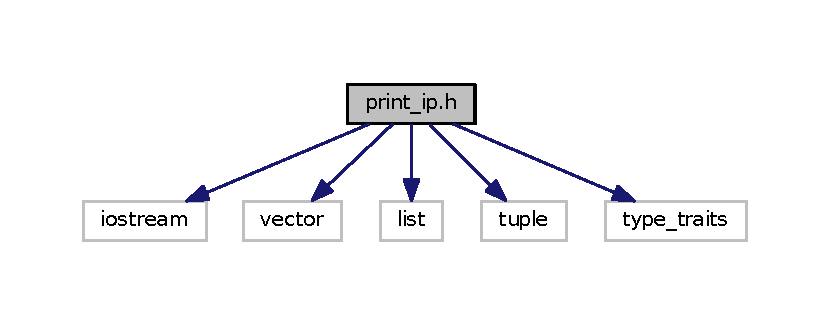
\includegraphics[width=350pt]{print__ip_8h__incl}
\end{center}
\end{figure}
This graph shows which files directly or indirectly include this file\+:
\nopagebreak
\begin{figure}[H]
\begin{center}
\leavevmode
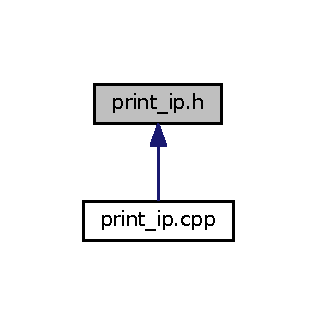
\includegraphics[width=152pt]{print__ip_8h__dep__incl}
\end{center}
\end{figure}
\subsection*{Classes}
\begin{DoxyCompactItemize}
\item 
struct \hyperlink{structcontainer}{container$<$ typename $>$}
\item 
struct \hyperlink{structcontainer_3_01std_1_1vector_3_01T_00_01Args_8_8_8_01_4_01_4}{container$<$ std\+::vector$<$ T, Args... $>$ $>$}
\item 
struct \hyperlink{structcontainer_3_01std_1_1list_3_01T_00_01Args_8_8_8_01_4_01_4}{container$<$ std\+::list$<$ T, Args... $>$ $>$}
\item 
struct \hyperlink{structis__valid}{is\+\_\+valid$<$ T, tuple\+\_\+args $>$}
\item 
struct \hyperlink{structis__valid_3_01T_00_01U_00_01tuple__args_8_8_8_01_4}{is\+\_\+valid$<$ T, U, tuple\+\_\+args... $>$}
\item 
struct \hyperlink{structis__valid_3_01T_00_01T_00_01tuple__args_8_8_8_01_4}{is\+\_\+valid$<$ T, T, tuple\+\_\+args... $>$}
\item 
struct \hyperlink{structis__valid_3_01T_00_01U_01_4}{is\+\_\+valid$<$ T, U $>$}
\item 
struct \hyperlink{structis__valid_3_01T_00_01T_01_4}{is\+\_\+valid$<$ T, T $>$}
\item 
struct \hyperlink{structis__valid_3_01T_01_4}{is\+\_\+valid$<$ T $>$}
\begin{DoxyCompactList}\small\item\em thank\textquotesingle{}s cxx17 standard \end{DoxyCompactList}\end{DoxyCompactItemize}
\subsection*{Functions}
\begin{DoxyCompactItemize}
\item 
void \hyperlink{print__ip_8h_ab85a39e729dc1b3396a77a5da5345dcd}{ip\+\_\+printer} (const std\+::string \&str)
\item 
{\footnotesize template$<$typename \+\_\+\+\_\+container $>$ }\\std\+::enable\+\_\+if\+\_\+t$<$ \hyperlink{structcontainer}{container}$<$ \+\_\+\+\_\+container $>$\+::value, void $>$ \hyperlink{print__ip_8h_a229cf5a6abbb8313fa417226fb072cba}{ip\+\_\+printer} (const \+\_\+\+\_\+container \&t)
\item 
{\footnotesize template$<$typename \+\_\+var\+\_\+arg $>$ }\\std\+::enable\+\_\+if\+\_\+t$<$ std\+::is\+\_\+integral\+\_\+v$<$ \+\_\+var\+\_\+arg $>$, void $>$ \hyperlink{print__ip_8h_a4fbfe43708e3a02818258687cb35da02}{ip\+\_\+printer} (const \+\_\+var\+\_\+arg t)
\item 
{\footnotesize template$<$typename... ts$>$ }\\std\+::enable\+\_\+if\+\_\+t$<$ \hyperlink{structis__valid}{is\+\_\+valid}$<$ ts... $>$\+::value, void $>$ \hyperlink{print__ip_8h_a6a08563005b5786b16d6281301500f20}{ip\+\_\+printer} (const std\+::tuple$<$ ts... $>$ \&\hyperlink{print__ip_8cpp_ae9ae314de04458b92af76712b52f71c8}{\+\_\+tuple})
\item 
{\footnotesize template$<$typename... ts$>$ }\\std\+::enable\+\_\+if\+\_\+t$<$ \hyperlink{structis__valid}{is\+\_\+valid}$<$ ts... $>$\+::value==false, void $>$ \hyperlink{print__ip_8h_afaab24dcc9f9e553b7ff61800dc0ccfb}{ip\+\_\+printer} (const std\+::tuple$<$ ts... $>$ \&\hyperlink{print__ip_8cpp_ae9ae314de04458b92af76712b52f71c8}{\+\_\+tuple})
\end{DoxyCompactItemize}


\subsection{Function Documentation}
\index{print\+\_\+ip.\+h@{print\+\_\+ip.\+h}!ip\+\_\+printer@{ip\+\_\+printer}}
\index{ip\+\_\+printer@{ip\+\_\+printer}!print\+\_\+ip.\+h@{print\+\_\+ip.\+h}}
\subsubsection[{\texorpdfstring{ip\+\_\+printer(const std\+::string \&str)}{ip_printer(const std::string &str)}}]{\setlength{\rightskip}{0pt plus 5cm}void ip\+\_\+printer (
\begin{DoxyParamCaption}
\item[{const std\+::string \&}]{str}
\end{DoxyParamCaption}
)}\hypertarget{print__ip_8h_ab85a39e729dc1b3396a77a5da5345dcd}{}\label{print__ip_8h_ab85a39e729dc1b3396a77a5da5345dcd}
\index{print\+\_\+ip.\+h@{print\+\_\+ip.\+h}!ip\+\_\+printer@{ip\+\_\+printer}}
\index{ip\+\_\+printer@{ip\+\_\+printer}!print\+\_\+ip.\+h@{print\+\_\+ip.\+h}}
\subsubsection[{\texorpdfstring{ip\+\_\+printer(const \+\_\+\+\_\+container \&t)}{ip_printer(const __container &t)}}]{\setlength{\rightskip}{0pt plus 5cm}template$<$typename \+\_\+\+\_\+container $>$ std\+::enable\+\_\+if\+\_\+t$<${\bf container}$<$\+\_\+\+\_\+container$>$\+::value,void$>$ ip\+\_\+printer (
\begin{DoxyParamCaption}
\item[{const \+\_\+\+\_\+container \&}]{t}
\end{DoxyParamCaption}
)}\hypertarget{print__ip_8h_a229cf5a6abbb8313fa417226fb072cba}{}\label{print__ip_8h_a229cf5a6abbb8313fa417226fb072cba}
\index{print\+\_\+ip.\+h@{print\+\_\+ip.\+h}!ip\+\_\+printer@{ip\+\_\+printer}}
\index{ip\+\_\+printer@{ip\+\_\+printer}!print\+\_\+ip.\+h@{print\+\_\+ip.\+h}}
\subsubsection[{\texorpdfstring{ip\+\_\+printer(const \+\_\+var\+\_\+arg t)}{ip_printer(const _var_arg t)}}]{\setlength{\rightskip}{0pt plus 5cm}template$<$typename \+\_\+var\+\_\+arg $>$ std\+::enable\+\_\+if\+\_\+t$<$std\+::is\+\_\+integral\+\_\+v$<$\+\_\+var\+\_\+arg$>$,void$>$ ip\+\_\+printer (
\begin{DoxyParamCaption}
\item[{const \+\_\+var\+\_\+arg}]{t}
\end{DoxyParamCaption}
)}\hypertarget{print__ip_8h_a4fbfe43708e3a02818258687cb35da02}{}\label{print__ip_8h_a4fbfe43708e3a02818258687cb35da02}
\index{print\+\_\+ip.\+h@{print\+\_\+ip.\+h}!ip\+\_\+printer@{ip\+\_\+printer}}
\index{ip\+\_\+printer@{ip\+\_\+printer}!print\+\_\+ip.\+h@{print\+\_\+ip.\+h}}
\subsubsection[{\texorpdfstring{ip\+\_\+printer(const std\+::tuple$<$ ts... $>$ \&\+\_\+tuple)}{ip_printer(const std::tuple< ts... > &_tuple)}}]{\setlength{\rightskip}{0pt plus 5cm}template$<$typename... ts$>$ std\+::enable\+\_\+if\+\_\+t$<${\bf is\+\_\+valid}$<$ts...$>$\+::value,void$>$ ip\+\_\+printer (
\begin{DoxyParamCaption}
\item[{const std\+::tuple$<$ ts... $>$ \&}]{\+\_\+tuple}
\end{DoxyParamCaption}
)}\hypertarget{print__ip_8h_a6a08563005b5786b16d6281301500f20}{}\label{print__ip_8h_a6a08563005b5786b16d6281301500f20}
\index{print\+\_\+ip.\+h@{print\+\_\+ip.\+h}!ip\+\_\+printer@{ip\+\_\+printer}}
\index{ip\+\_\+printer@{ip\+\_\+printer}!print\+\_\+ip.\+h@{print\+\_\+ip.\+h}}
\subsubsection[{\texorpdfstring{ip\+\_\+printer(const std\+::tuple$<$ ts... $>$ \&\+\_\+tuple)}{ip_printer(const std::tuple< ts... > &_tuple)}}]{\setlength{\rightskip}{0pt plus 5cm}template$<$typename... ts$>$ std\+::enable\+\_\+if\+\_\+t$<${\bf is\+\_\+valid}$<$ts...$>$\+::value == false,void$>$ ip\+\_\+printer (
\begin{DoxyParamCaption}
\item[{const std\+::tuple$<$ ts... $>$ \&}]{\+\_\+tuple}
\end{DoxyParamCaption}
)}\hypertarget{print__ip_8h_afaab24dcc9f9e553b7ff61800dc0ccfb}{}\label{print__ip_8h_afaab24dcc9f9e553b7ff61800dc0ccfb}

\hypertarget{README_8md}{}\section{R\+E\+A\+D\+M\+E.\+md File Reference}
\label{README_8md}\index{R\+E\+A\+D\+M\+E.\+md@{R\+E\+A\+D\+M\+E.\+md}}

\hypertarget{test__version_8cpp}{}\section{test\+\_\+version.\+cpp File Reference}
\label{test__version_8cpp}\index{test\+\_\+version.\+cpp@{test\+\_\+version.\+cpp}}
{\ttfamily \#include \char`\"{}version\+\_\+lib.\+h\char`\"{}}\\*
{\ttfamily \#include $<$boost/test/unit\+\_\+test.\+hpp$>$}\\*
Include dependency graph for test\+\_\+version.\+cpp\+:
\nopagebreak
\begin{figure}[H]
\begin{center}
\leavevmode
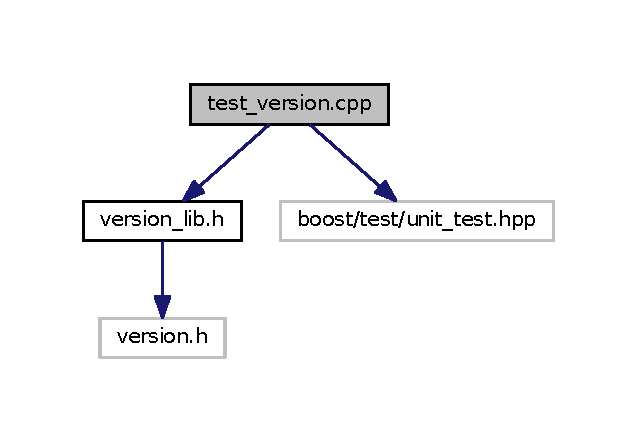
\includegraphics[width=306pt]{test__version_8cpp__incl}
\end{center}
\end{figure}
\subsection*{Macros}
\begin{DoxyCompactItemize}
\item 
\#define \hyperlink{test__version_8cpp_a6b2a3852db8bb19ab6909bac01859985}{B\+O\+O\+S\+T\+\_\+\+T\+E\+S\+T\+\_\+\+M\+O\+D\+U\+LE}~helloworld\+\_\+test\+\_\+module
\end{DoxyCompactItemize}
\subsection*{Functions}
\begin{DoxyCompactItemize}
\item 
\hyperlink{test__version_8cpp_a3b04136cdb86770b6bf5f3fc478d9f3f}{B\+O\+O\+S\+T\+\_\+\+A\+U\+T\+O\+\_\+\+T\+E\+S\+T\+\_\+\+C\+A\+SE} (alloc\+\_\+test\+\_\+version)
\end{DoxyCompactItemize}


\subsection{Macro Definition Documentation}
\index{test\+\_\+version.\+cpp@{test\+\_\+version.\+cpp}!B\+O\+O\+S\+T\+\_\+\+T\+E\+S\+T\+\_\+\+M\+O\+D\+U\+LE@{B\+O\+O\+S\+T\+\_\+\+T\+E\+S\+T\+\_\+\+M\+O\+D\+U\+LE}}
\index{B\+O\+O\+S\+T\+\_\+\+T\+E\+S\+T\+\_\+\+M\+O\+D\+U\+LE@{B\+O\+O\+S\+T\+\_\+\+T\+E\+S\+T\+\_\+\+M\+O\+D\+U\+LE}!test\+\_\+version.\+cpp@{test\+\_\+version.\+cpp}}
\subsubsection[{\texorpdfstring{B\+O\+O\+S\+T\+\_\+\+T\+E\+S\+T\+\_\+\+M\+O\+D\+U\+LE}{BOOST_TEST_MODULE}}]{\setlength{\rightskip}{0pt plus 5cm}\#define B\+O\+O\+S\+T\+\_\+\+T\+E\+S\+T\+\_\+\+M\+O\+D\+U\+LE~helloworld\+\_\+test\+\_\+module}\hypertarget{test__version_8cpp_a6b2a3852db8bb19ab6909bac01859985}{}\label{test__version_8cpp_a6b2a3852db8bb19ab6909bac01859985}


\subsection{Function Documentation}
\index{test\+\_\+version.\+cpp@{test\+\_\+version.\+cpp}!B\+O\+O\+S\+T\+\_\+\+A\+U\+T\+O\+\_\+\+T\+E\+S\+T\+\_\+\+C\+A\+SE@{B\+O\+O\+S\+T\+\_\+\+A\+U\+T\+O\+\_\+\+T\+E\+S\+T\+\_\+\+C\+A\+SE}}
\index{B\+O\+O\+S\+T\+\_\+\+A\+U\+T\+O\+\_\+\+T\+E\+S\+T\+\_\+\+C\+A\+SE@{B\+O\+O\+S\+T\+\_\+\+A\+U\+T\+O\+\_\+\+T\+E\+S\+T\+\_\+\+C\+A\+SE}!test\+\_\+version.\+cpp@{test\+\_\+version.\+cpp}}
\subsubsection[{\texorpdfstring{B\+O\+O\+S\+T\+\_\+\+A\+U\+T\+O\+\_\+\+T\+E\+S\+T\+\_\+\+C\+A\+S\+E(alloc\+\_\+test\+\_\+version)}{BOOST_AUTO_TEST_CASE(alloc_test_version)}}]{\setlength{\rightskip}{0pt plus 5cm}B\+O\+O\+S\+T\+\_\+\+A\+U\+T\+O\+\_\+\+T\+E\+S\+T\+\_\+\+C\+A\+SE (
\begin{DoxyParamCaption}
\item[{alloc\+\_\+test\+\_\+version}]{}
\end{DoxyParamCaption}
)}\hypertarget{test__version_8cpp_a3b04136cdb86770b6bf5f3fc478d9f3f}{}\label{test__version_8cpp_a3b04136cdb86770b6bf5f3fc478d9f3f}

\hypertarget{version_8h}{}\section{version.\+h File Reference}
\label{version_8h}\index{version.\+h@{version.\+h}}
This graph shows which files directly or indirectly include this file\+:
\nopagebreak
\begin{figure}[H]
\begin{center}
\leavevmode
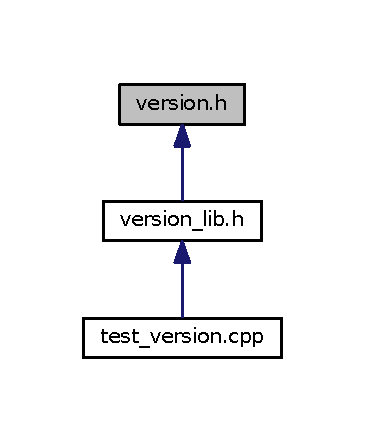
\includegraphics[width=175pt]{version_8h__dep__incl}
\end{center}
\end{figure}
\subsection*{Macros}
\begin{DoxyCompactItemize}
\item 
\#define \hyperlink{version_8h_a4a5fc96a4bdd7d68ed99ccce9ca2e77e}{P\+R\+O\+J\+E\+C\+T\+\_\+\+V\+E\+R\+S\+I\+O\+N\+\_\+\+P\+A\+T\+CH}~17
\end{DoxyCompactItemize}


\subsection{Macro Definition Documentation}
\index{version.\+h@{version.\+h}!P\+R\+O\+J\+E\+C\+T\+\_\+\+V\+E\+R\+S\+I\+O\+N\+\_\+\+P\+A\+T\+CH@{P\+R\+O\+J\+E\+C\+T\+\_\+\+V\+E\+R\+S\+I\+O\+N\+\_\+\+P\+A\+T\+CH}}
\index{P\+R\+O\+J\+E\+C\+T\+\_\+\+V\+E\+R\+S\+I\+O\+N\+\_\+\+P\+A\+T\+CH@{P\+R\+O\+J\+E\+C\+T\+\_\+\+V\+E\+R\+S\+I\+O\+N\+\_\+\+P\+A\+T\+CH}!version.\+h@{version.\+h}}
\subsubsection[{\texorpdfstring{P\+R\+O\+J\+E\+C\+T\+\_\+\+V\+E\+R\+S\+I\+O\+N\+\_\+\+P\+A\+T\+CH}{PROJECT_VERSION_PATCH}}]{\setlength{\rightskip}{0pt plus 5cm}\#define P\+R\+O\+J\+E\+C\+T\+\_\+\+V\+E\+R\+S\+I\+O\+N\+\_\+\+P\+A\+T\+CH~17}\hypertarget{version_8h_a4a5fc96a4bdd7d68ed99ccce9ca2e77e}{}\label{version_8h_a4a5fc96a4bdd7d68ed99ccce9ca2e77e}

\hypertarget{version__lib_8h}{}\section{version\+\_\+lib.\+h File Reference}
\label{version__lib_8h}\index{version\+\_\+lib.\+h@{version\+\_\+lib.\+h}}
{\ttfamily \#include \char`\"{}version.\+h\char`\"{}}\\*
Include dependency graph for version\+\_\+lib.\+h\+:
\nopagebreak
\begin{figure}[H]
\begin{center}
\leavevmode
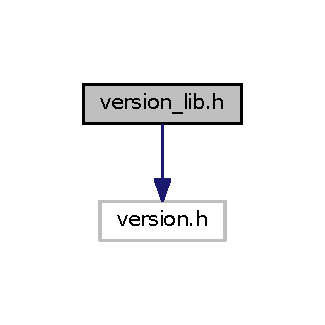
\includegraphics[width=156pt]{version__lib_8h__incl}
\end{center}
\end{figure}
This graph shows which files directly or indirectly include this file\+:
\nopagebreak
\begin{figure}[H]
\begin{center}
\leavevmode
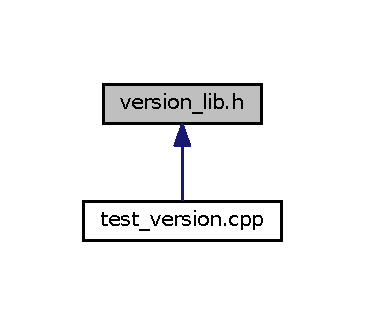
\includegraphics[width=175pt]{version__lib_8h__dep__incl}
\end{center}
\end{figure}
\subsection*{Functions}
\begin{DoxyCompactItemize}
\item 
int \hyperlink{version__lib_8h_ae64f17a84dc9c7144d1036498ff26fd9}{version} ()
\end{DoxyCompactItemize}


\subsection{Function Documentation}
\index{version\+\_\+lib.\+h@{version\+\_\+lib.\+h}!version@{version}}
\index{version@{version}!version\+\_\+lib.\+h@{version\+\_\+lib.\+h}}
\subsubsection[{\texorpdfstring{version()}{version()}}]{\setlength{\rightskip}{0pt plus 5cm}int version (
\begin{DoxyParamCaption}
{}
\end{DoxyParamCaption}
)}\hypertarget{version__lib_8h_ae64f17a84dc9c7144d1036498ff26fd9}{}\label{version__lib_8h_ae64f17a84dc9c7144d1036498ff26fd9}

%--- End generated contents ---

% Index
\backmatter
\newpage
\phantomsection
\clearemptydoublepage
\addcontentsline{toc}{chapter}{Index}
\printindex

\end{document}
